\chapter{Computational Model}\label{ch:computational}

\textcolor{red}{FINAL - TO BE READ ONE LAST TIME}

In this chapter, we propose \river{}\footnote{The name \river, and its graphics, is inspired by the data continuously flowing one way into the system.} -- a variety-proof computational model to deal with streaming data.
Section~\ref{sec:comp-mod-intro} introduces the problem of dealing with data characterized by high \textit{Variety} and \textit{Velocity} without forgetting \textit{Volume}.
In Section~\ref{sec:comp-mod-sol}, we propose a) the background concepts that underpin \river{}, b) the semantics and textual syntax of the operators of \river{} and c) the Pipeline Definition Language -- a graphic language to ease the modeling of \river{} plans.

\section{Introduction and Problem Statement} \label{sec:comp-mod-intro}
In our case studies (see Chapter~\ref{ch:case-studies}), we noticed that data can come from different sources that vary in format (\textit{Variety}) and size (\textit{Volume}), but it  always flows (\textit{Velocity}). Even what we normally call "\textit{static data}", e.g.,  a city street network, is not immutable over time, it  slowly evolves.

In 2013, we presented SLD (see Section~\ref{sec:rsp-mid}), a middleware to ease the deployment of an RSP engine in a real world scenario characterized by heterogeneous streaming data.
In five years of SLD usage, we learned that using RDF streams is valuable when (i) data are naturally represented as graphs, (e.g., micro-posts in the larger social graph) and when (ii) the availability of popular vocabularies eases the development of adapters that semantically annotate the external data flows.
For instance, we wrote adapters that annotate streams from the major social networks using SIOC~\cite{DBLP:journals/ijwbc/BreslinDHB06}.

However, we also found out several weaknesses of the RDF-only approach: (i) RDF streams cannot be found in the wild, yet, JSON is largely used in practice (e.g., Twitter Streaming APIs\footnote{\url{https://dev.twitter.com/streaming/overview}} and W3C activity stream 2.0 working draft\footnote{\url{http://www.w3.org/TR/activitystreams-core/}}) and (ii) the results of a continuous computation are often relational and forcing them into an RDF stream is suboptimal.
%(e.g., a user would naturally use the REGISTER QUERY ... AS SELECT ... form instead of REGISTER STREAM ... AS CONSTRUCT ... one. It takes three triples to state how many times a hashtag appears in the micro-posts observed in 1 minute, while the tuple $\langle$timestamp, hashtag, count$\rangle$ is more succinct).

Those reflections inspired the idea to work with the data in its original format as long as possible to reduce the latency caused by the data transformations at ingestion time. We named this approach \textit{Lazy Transformation}.

In order to investigate how \textit{Lazy Transformation} helps in address our research questions -- \textit{Is it possible to continuously ingest and reactively analyses a variety of streaming urban data in order to visualize emerging patterns and their dynamics?} -- we formulate the hypothesis:

\begin{itemize}[leftmargin=42pt]
\item[\textsf{Hp.2.1}] The implementation of a streaming computational model that defers as long as possible the data transformation demands less resources and better approximates the correct answer under stress conditions than an implementation of a computational model that cast data into RDF at ingestion time.
\end{itemize}

\section{\texorpdfstring{\protect\river{}}{RIVER}}\label{sec:comp-mod-sol}
In the next sections, we present \river{}, a variety proof streaming computational model built around the idea of \textit{Lazy Transformation}.

In Section~\ref{sec:comp-mod-sol-pre}, we introduce the background concepts that underpin \river{}.
Section~\ref{sec:comp-mod-sol-lang} presents in detail the semantics and the textual syntaxes of the \river{}'s operators, the Pipeline Definition Language (PDL) -- a graphic syntax to abstract the implementation complexity -- and, eventually, examples of physical languages (e.g., EPL, SQL, SPARQL, etc.) to implement the \river{}'s operators. All of those concepts are presented through a running example.
Finally, in Section~\ref{sec:comp-mod-sol-arch}, we present a reference architecture for systems that implement \river{}.

\subsection{Preliminaries}\label{sec:comp-mod-sol-pre}
Based on the considerations resulting from the development of our conceptual model (see Chapter~\ref{ch:conceptual}) and on our past experiences (see Chapter~\ref{ch:case-studies}), we identify two principles that inspire \river{}.

\textbf{(P1)} \textit{Everything is a data stream}. According to this principle, a variety-proof stream processing engine must indifferently ingest data with different velocities from any sources and of any size. 

For instance, the movements of a car is a \textit{fast} data stream where the information flow records the identity, the positions and the speeds of the cars. In this case, the distance between two subsequent observations can be seconds. On the other side, a city road is a \textit{slowly evolving} data stream, where the information flow contains, for instance, the information about the addition of a bike lane.
In this second case, the distance between two subsequent observations can be days or months. 

The continuous nature of data streams, and the importance of the information extracted by the most fresh data, require such a category of engine to avoid data loss and, consequently, to implement our second principle: \textbf{(P2)} \textit{Continuous Ingestion}. The data in input is continuously captured by the system and, once arrived, it is marked with an increasing timestamp. Notably, some data sources may natively include their own timestamp too (namely, the application timestamp, presented in Section~\ref{sec:secret}). It is worth to note that a continuous ingestion mechanism helps to avoid data losses, but continuous analysis is not always needed; an analysis can be reactive even if postponed (see Section~\ref{sec:comp-mod-eval-cost}).

In order to challenge the hypothesis \textsf{Hp.2.1}, we propose the \textit{Lazy Transformation} approach. 
A variety-proof stream processing engine operates on the data in its original format as long as it can, and it transforms data only if it really needs to do so. Indeed, operations like projections, filters or aggregations can operate on generic data without requiring to cast all data in a single format (such as RDF). Therefore, for those operations, we can delay transformations. Contrariwise, a join operation, normally, first requires to cast data in a common format (e.g., the relational one). 

So, this kind of system must rely on data of generic type $\mathrm{T}$.

\begin{Definition}
(Type to-be-specified-later) A type to-be-specified-later $\mathrm{T}$ represents the generic type of the atomic object flowing into the system.
\end{Definition}

Together with the definition of time (already reported in Section~\ref{sec:stream-proc}), we can define the information flowing into this kind of systems as a Generic Data Stream.

\begin{Definition}
(Time) The time $\mathcal{T}$ is an infinite, discrete, ordered sequence of time instants $(\tau_1,\tau_2,..., \tau_n)$, where $\tau_i \in \mathbb{N}$. A time unit is the difference between two consecutive time instants $(\tau_{i+1} - \tau_i)$ and it is constant.
\end{Definition}

\begin{Definition}
(Generic Data Stream) A Generic Data Stream S$\langle\mathrm{T}\rangle$ is a potentially unbounded sequence of timestamped data items $(d_i,\tau_i)$:
\noindent\begin{align*}
S = (d_1,\tau_1), (d_2,\tau_2), \ldots, (d_n,\tau_n)
\end{align*}  
where $d_i$ is of type $\mathrm{T}$, $\tau_i \in \mathcal{T}$ is the associated time instant and $\tau_i<\tau_{i+1}$.
\end{Definition}

Note that the time instants associated to data items is monotonically increasing. We do not allow contemporary ingestion, because we consider the time as a form of punctuation. 
So, the data items $d_i$ in a Generic Data Stream S$\langle\mathrm{T}\rangle$ is of \textit{types to-be-specified-later} $\mathrm{T}$, and, for instance, it can be, indifferently, a tree representation of a JSON document, a set of tuples in CSV or in parquet format, or a graph in RDF.

\textit{Generic Functions} and \textit{Generic Types}~\cite{DBLP:conf/dagstuhl/1998gp} represents the natural abstraction to model the operations that manipulate information in accordance with the \textit{Lazy Transformation} approach. 

Let us now define a Generic Time-Varying Collection as:

\begin{Definition}
(Generic Time-Varying Collection) A Generic Time-Varying Collection C$\langle\mathrm{T}\rangle$ is a mapping from $\mathcal{T}$ to a finite but unbounded bag of data items $d_i$, where $d_i$ is of type $\mathrm{T}$. 
\end{Definition}

Differently from a Generic Time-Varying Collection, a Generic Instantaneous Collection defines an unordered bag of data items at a specific time instant.

\begin{Definition}
(Generic Instantaneous Collection) A Generic Instantaneous Collection  C$\langle\mathrm{T}\rangle(\tau)$ is the bag of data items in a collection at $\tau$, a given point in time . 
\end{Definition}

\subsection{\texorpdfstring{\protect\river{}}{RIVER}'s Operators and the Pipeline Definition Language}\label{sec:comp-mod-sol-lang}

\river{} computational model enables users to define computational plans, in the form of pipelines (formally DAGs\footnote{A finite directed graph with no directed cycles.}), composed by different operators that take care of ingesting, processing and emitting Generic Data Streams.
In order to ease the definition of the computational plans, we propose the Pipeline Definition Language (PDL).
It defines the graphical syntax of the operators.

\begin{figure}[t]
  \centering
  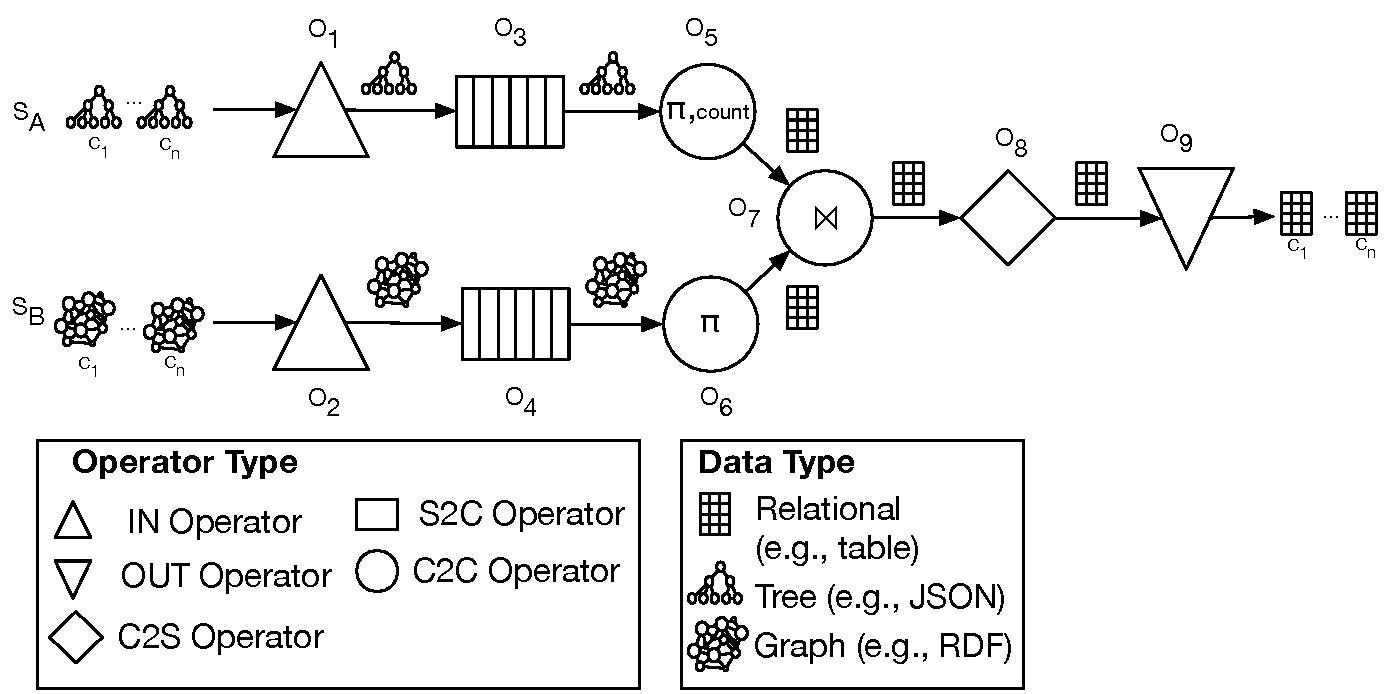
\includegraphics[width=0.92\textwidth]{img/computational-model-syntax-example-ODL}
  \caption{Pipeline that presents an example of the operators and of the typical data type produced during the computation.}
  \label{fig:sti_ex}
\end{figure} 

The reader will be guided into the details via the running example depicted in Figure~\ref{fig:sti_ex}.
The presented operators and symbols will be detailed discussed in the next paragraphs.

\begin{Example}
The example, depicted in Figure~\ref{fig:sti_ex}, represents the pipeline to deal with a typical social media analytics use case.
The inputs to the pipeline are the post stream S$_A$ and the users' friend network, the stream S$_B$, in the form of graph. The two streams have to be joined in order to connect users with common friends in the same location.
\end{Example}
 
More formally, Figure~\ref{fig:cm-op} depicts the five classes of \river{} operators and their interactions. 
The operators, defined as S2C$\langle\mathrm{T}\rangle$, C2C$\langle\mathrm{T},\mathrm{T^{\prime}}\rangle$ and C2S$\langle\mathrm{T}\rangle$ in \river{}, are inspired to the CQL processing model (see Section~\ref{sec:CQL}), and allow to move from S$\langle\mathrm{T}\rangle$ to C$\langle\mathrm{T}\rangle$ and vice-versa.
In addition to the CQL-like operators, we introduce the \textit{ingestion} (defined as IN$\langle\mathrm{T}\rangle$ in \river{}) and \textit{emission} (defined as OUT$\langle\mathrm{T}\rangle$ in \river{}) operators.
They, respectively, ingest and emit external data flow to/from a system implemented using \river{} computational model.

In the next paragraphs, we report the details of the operators and present, for each of them, its formal definition, its graphical syntax in PDL, the examples of physical languages for its implementation and its role in the running example (see Figure~\ref{fig:sti_ex}).

\begin{figure}[t]
    \centering
    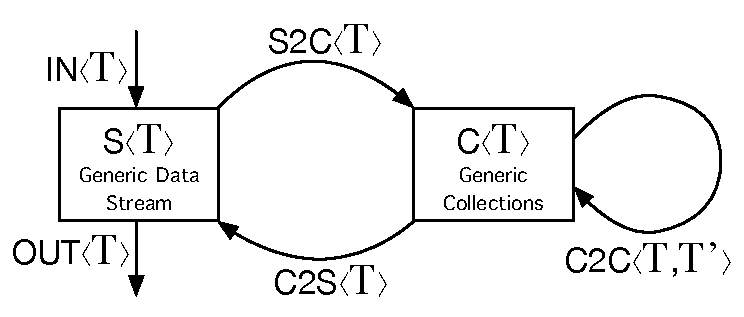
\includegraphics[width=0.8\textwidth]{img/computational-model-operators}
    \caption{Overview of \textnormal{\protect\river{}} operators.}
    \label{fig:cm-op}
\end{figure}

\medskip
\noindent
\textbf{Ingestion Operator}
\medskip

\begin{Definition}
(Ingestion operator) A IN$\langle\mathrm{T}\rangle$ operator takes an external data flow and inject the items into the system creating a new S$\langle\mathrm{T}\rangle$. 
The ingestion operator is type-agnostic, it works independently from the external source data-type.
It always transform the items in the external data flow into internal generics (defined as $\langle\mathrm{T}\rangle$).
\end{Definition}

\noindent
In PDL we introduce the symbol $\bigtriangleup$ to represent the Ingestion operator.

\begin{Example}
(cont'd) The external data flows S$_A$ and S$_B$ need to be ingested in order to be analyzed.
O$_1$ and O$_2$ are implementations of IN$\langle\mathrm{T}\rangle$ operator for Twitter. 
They contain the logic for connecting to twitter and retrieve the requested informations.
On the one hand, O$_1$ takes care of the external data flow S$_A$, by connecting to the Twitter streaming API and ingesting JSON Trees as generics $\langle\mathrm{T}\rangle$.
Listing~\ref{lst:o1_res} shows the resulting JSON.

\begin{figure}[ht]
\begin{minipage}{0.95\linewidth}
\begin{lstlisting}[caption={Example of the data resulting by the ingestion operation performed by O$_1$.},label=lst:o1_res,style=JSON]
  {
    "data": [{
      "user_id": ":Alice",
      "content": "breathless at #moma",
      "hashtag": [
         { 
           "tag_id":"t1"
           "text":"moma"
         }
      ],
      "latitude":40.761620,
      "longitude":-73.977257,
      "time":"2018-09-30T09:00:00"
     }
    ]
   }
\end{lstlisting}
\end{minipage}
\end{figure}

On the other hand, O$_1$ manages the external data flow S$_B$, by polling the Twitter REST API and ingesting RDF Graph as generics $\langle\mathrm{T}\rangle$.
Listing~\ref{lst:o2_res} shows the resulting RDF Graph.

\begin{figure}[ht]
\begin{minipage}{0.95\linewidth}
\begin{lstlisting}[caption={Example of the data resulting by the ingestion operation performed by O$_2$.},label=lst:o2_res,style=N3]
:Alice a :User ;
    :userName "Alice"^^xsd:string ;
    :birthDate "1980-06-21"^^xsd:date ;
    :hasFriend :Bob .
\end{lstlisting}
\end{minipage}
\end{figure}

\end{Example}

\medskip
\noindent
\textbf{Stream-to-collection Operator}
\medskip

\begin{Definition}
(Stream-to-collection operator) A S2C$\langle\mathrm{T}\rangle$ operator transforms a portion of a potentially infinite Generic Data Stream S$\langle\mathrm{T}\rangle$ into a Generic Time-Varying Collection C$\langle\mathrm{T}\rangle$.
S2C$\langle\mathrm{T}\rangle$ operator is type-agnostic, the operation is completely independent from $\mathrm{T}$.
\end{Definition}

Similarly to CQL, the implementations of the S2C$\langle\mathrm{T}\rangle$ operator are based on the concept of \textit{sliding window}.
In particular, we can define the concept of Generic Data Window.

\begin{Definition}
(Generic Data Window) A window W$\langle\mathrm{T}\rangle(S)$ is a set of data items (d$_1$, ..., d$_n$), of type $\mathrm{T}$, extracted from a Generic Data Stream S$\langle\mathrm{T}\rangle$. 
\end{Definition}

Exploiting this concept we can now define two classes of Generic Data Window.
The \textit{time-based} Sliding Generic Data Window and the \textit{tuple-based} Generic Data Window.

Time-based Sliding Generic Data Window operator defines its output by sliding an interval of $\mathrm{K}$ time units over the stream S$\langle\mathrm{T}\rangle$.

\begin{Definition}
(Time-based Sliding Generic Data Window) A Time-based Sliding Generic Data Window on a stream S$\langle\mathrm{T}\rangle$ takes a time-interval $\mathrm{K}$ as a parameter and is specified by following S$\langle\mathrm{T}\rangle$ in the query with [Range $\mathrm{K}$].
The output Generic Instantaneous Collection C$\langle\mathrm{T}\rangle(\tau)$ of S$\langle\mathrm{T}\rangle$[Range $\mathrm{K}$] is defined as:
\noindent\begin{align*}
C\langle\mathrm{T}\rangle(\tau)=\{s \mid \langle s,\tau' \rangle \in S\langle\mathrm{T}\rangle \wedge (\tau' \leq \tau) \wedge (\tau' \geq \max\{\tau - \mathrm{K},0\})\}
\end{align*}  
\end{Definition}

Tuple-based Sliding Generic Data Window operator defines its output by sliding a window of size $\mathrm{N}$ data items over the stream S$\langle\mathrm{T}\rangle$.
\begin{Definition}
(Tuple-based Sliding Generic Data Window) A Tuple-based Sliding Generic Data Window takes a positive integer $\mathrm{N}$ as a parameter and is specified by following S$\langle\mathrm{T}\rangle$ in the query with [Rows $\mathrm{N}$].
The Generic Instantaneous Collection C$\langle\mathrm{T}\rangle(\tau)$ of S$\langle\mathrm{T}\rangle$[Rows $\mathrm{N}$], consists of data items of type $\mathrm{T}$ obtained from the $\mathrm{N}$ elements with the largest timestamps in S$\langle\mathrm{T}\rangle$ no greater than $\tau$.
\end{Definition}

%Partitioned Sliding Generic Data Window logically partitions S$\langle\mathrm{T}\rangle$ into sub-streams based on equality of attributes $A_1, ..., A_k$, computes a Tuple-based Sliding Generic Data Window of size $N$ on each sub-stream, then produce a Generic Collection which contains the union of these sub-windows.

%\begin{Definition}
%(Partitioned Sliding Generic Data Window) A Partitioned Sliding Generic Data Window on a stream S$\langle\mathrm{T}\rangle$ takes a positive integer N and a subset $\{A_1, ..., A_k\}$ of S attributes as parameters. It is specified by following S$\langle\mathrm{T}\rangle$ in the query with [Partition By $A_1, ..., A_k$ Rows N].
%Formally, a data item d of type $\mathrm{T}$ with values $a_1, ..., a_k$ for attributes $A_1, ..., A_k$ occurs in output Generic Instantaneous Collection C$\langle\mathrm{T}\rangle(\tau)$ iff exists an element $\langle d,\tau' \rangle \in S\langle\mathrm{T}\rangle$ such that $\tau' \leq \tau$ is among the N largest timestamps among elements whose tuples have values $a_1, ..., a_k$ for attributes $A_1, ..., A_k$
%\end{Definition}

\noindent
In PDL, we use the symbol $\hrectangle$ to represent the S2C$\langle\mathrm{T}\rangle$ operator. 
In particular, the symbol related to the S2C$\langle\mathrm{T}\rangle$ operators can give an hint about the operator's implementation.
For instance, the S2C$\langle\mathrm{T}\rangle$ operators O$_3$ and O$_4$, proposed in Figure~\ref{fig:sti_ex}, are implemented as two windowers.

\begin{Example}
(cont'd) The operators O$_3$ and O$_4$ apply Time-based sliding window operations to the streams resulting from the operators O$_1$ and O$_2$.
Operator O$_3$ is a S2C$\langle Tree \rangle$, while O$_4$ implements a S2C$\langle Graph \rangle$

As anticipated in the introduction, we report the physical implementation of some operators. 
In this case, both O$_3$ and O$_4$ can be implemented exploiting ESPER engine (see Section~\ref{sec:esper-epl}) and using the EPL clause TIME to create sliding windows with 1 minute duration.
Note that the operators are completely agnostic to the data type. O$_3$ and O$_4$ are the same query, except for the name of the stream (see Linting~\ref{lst:epl-win-03} and Linting~\ref{lst:epl-win-04}).

\begin{figure}[ht]
\begin{minipage}{0.95\linewidth}
\begin{lstlisting}[caption={EPL query, applied by O$_3$ operator, to window the stream of JSON trees},label=lst:epl-win-03,style=ESPER]
     SELECT * FROM treeEvent#TIME(1 MIN) 
\end{lstlisting}
\end{minipage}
\end{figure}

\begin{figure}[ht]
\begin{minipage}{0.95\linewidth}
\begin{lstlisting}[caption={EPL query, applied by O$_4$ operator, to window the stream of RDF graphs},label=lst:epl-win-04,style=ESPER]
     SELECT * FROM graphEvent#TIME(1 MIN) 
\end{lstlisting}
\end{minipage}
\end{figure}

The proposed EPL queries, produce two Generic Instantaneous Collections that contain, respectively, the JSON trees and the RDF graphs ingested in the last minute, without apply any transformation to the data items.

\begin{figure}[p]
\begin{minipage}{0.95\linewidth}
\begin{lstlisting}[caption={Example of result of the O$_3$ operators.},label=lst:o3_res,style=JSON]
  {
    "data": [{
      "user_id": ":Alice",
      "content": "breathless at #moma",
      "hashtag": [
         { 
           "tag_id":"t1"
           "text":"moma"
         }
      ],
      "latitude":40.761620,
      "longitude":-73.977257,
      "time":"2018-09-30T09:00:00"
     },{
      "user_id": ":David",
      "content": "Morning at #moma",
      "hashtag": [
         { 
           "tag_id":"t1"
           "text":"moma"
         }
      ],
      "latitude":40.761620,
      "longitude":-73.977257,
      "time":"2018-09-30T09:00:30"
     },{
      "user_id": ":Carl",
      "content": "Spending my day at #MoMA",
      "hashtag": [
         { 
           "tag_id":"t2"
           "text":"MoMA"
         }
      ],
      "latitude":40.761620,
      "longitude":-73.977257,
      "time":"2018-09-30T09:00:45"
     },{
      "user_id": ":Alice",
      "content": "#picasso at #moma",
      "hashtag": [
         { 
           "tag_id":"t1"
           "text":"moma"
         }, { 
           "tag_id":"t3"
           "text":"picasso"
         }
      ],
      "latitude":40.761620,
      "longitude":-73.977257,
      "time":"2018-09-30T09:00:55"
     }
    ]
  }
\end{lstlisting}
\end{minipage}
\end{figure}

Before producing the output, in order to enable query operation for the downstream operators, O$_3$ merges the different JSON trees in a single JSON tree which contains an array of elements (see Listing~\ref{lst:o3_res}).
The operator O$_4$ works in a similar way on the input stream of RDF graphs. It windows the stream and creates a single RDF graph in output that contains all the information that entered the system in the last minute (see Listing~\ref{lst:o4_res}).

\begin{figure}[ht]
\begin{minipage}{0.95\linewidth}
\begin{lstlisting}[caption={Example of result of the O$_4$ operator.},label=lst:o4_res,style=N3]
:Alice a :User ;
    :userName "Alice"^^xsd:string ;
    :birthDate "1980-06-21"^^xsd:date ;
    :hasFriend :Bob .
:Bob a :User ;
    :userName "Bob"^^xsd:string ;
    :birthDate "1965-08-10"^^xsd:date ;
    :hasFriend :Alice ;
    :hasFriend :Carl .
:Carl a :User ;
    :userName "Carl"^^xsd:string ;
    :birthDate "1965-05-15"^^xsd:date ;
    :hasFriend :Bob .
\end{lstlisting}
\end{minipage}
\end{figure}

\end{Example}

\medskip
\noindent
\textbf{Collection-to-collection Operator}
\medskip

\begin{Definition}
(Collection-to-collection operator) A C2C$\langle\mathrm{T},\mathrm{T^{\prime}}\rangle)$ operator transforms one or more Generic Instantaneous Collection C$\langle\mathrm{T}\rangle(\tau)$ in input into a single Generic Instantaneous Collection C$\langle\mathrm{T'}\rangle(\tau)$.
\end{Definition}

The implementations of this class of operators are tailored on the different data format, e.g., JSONiq operators process  JSON,  SQL operators process relational table, SPARQL operators process RDF graph, etc. Notably, $\mathrm{T}$ and $\mathrm{T^{\prime}}$ can be of different types, but they can also be of the same type. For instance, a filter on a table, on a tree or on a graph extract tuples, sub-trees or sub-graphs maintaining the original data type. Contrariwise, as we noticed above, a count aggregation transform the original data type into a table.

\noindent
In PDL, we use the symbol $\bigcirc$ to represent the C2C$\langle\mathrm{T},\mathrm{T^{\prime}}\rangle$ operator.

\begin{Example}
(cont'd) The operator O$_5$ is a C2C$\langle Tree,Relational\rangle$ and performs an aggregation on the output of the O$_3$ operator. 
The JSON object from O$_3$ contains the list of the posts that have entered the system in the last minute.
Differently from the generic EPL queries (see Listing~\ref{lst:epl-win-03} and Listing~\ref{lst:epl-win-04}), in order to perform the aggregation query (presented in the Listing~\ref{lst:oc_query}) the operator O$_5$ needs to know the data format in advance. As specified in the operator's definition, the implementation of the operator change with the input data type and can be choose at design time.

\begin{figure}[ht]
\begin{minipage}{0.95\linewidth}
\begin{lstlisting}[caption={JSONiq Query for aggregating JSON element, applied by the operators O$_5$.},label=lst:oc_query,style=JSONIQ]
FOR $user IN COLLECTION("data")
GROUP BY $user_id := $user.user_id
RETURN { "user_id" : $user_id, "count" : COUNT($user) }
\end{lstlisting}
\end{minipage}
\end{figure}

The query in Listing~\ref{lst:oc_query} counts the elements in the list, grouped by user\_id, and produces a relational table. 

\begin{table}[ht]
\centering
\caption{Example of result produced by the O$_5$ operator.}
\label{tbl:oc_res}
    \begin{tabular}{|c|c|}
        \hline
        \textbf{user\_id} & \textbf{count} \\ \hline
        :Alice             & 2              \\ \hline
        :Carl              & 1              \\ \hline
        :David             & 1              \\ \hline
    \end{tabular}
\end{table}

Table~\ref{tbl:oc_res} presents the output of O$_5$: a relational table with the user\_id and the associated count.

In the other branch of the pipeline, which manage the slowly evolving data that enter the system in RDF graph format, the operator O$_6$, similarly to the operator O$_5$, extracts information related only to the users who have at least one friend in common.  

\begin{figure}[ht]
\begin{minipage}{0.95\linewidth}
\begin{lstlisting}[caption={SPAQL query applied by operator O$_6$ to the RDF stream to project information about the user.},label=lst:od_query,style=SPARQL]
SELECT ?user_id ?name ?birthDate
WHERE {
    ?user1 a :User;
    :user_id ?user_id ;
    :userName ?name ;
    :birthDate ?birthDate ;
    :hasFriend ?commonFriends .
    ?user2 a :User;
    :hasFriend ?commonFriends .    
FILTER (?user1 != ?user2)
} 
\end{lstlisting}
\end{minipage}
\end{figure}

\medskip

Operator O$_6$ is a C2C$\langle Graph,Relational\rangle$.
It extracts information from the slowly evolving RDF graph stream via the SPARQL query presented in Listing~\ref{lst:od_query} and creates a relational table as presented in the Table~\ref{tbl:od_res}.

\begin{table}[ht]
\centering
\caption{Example of result produced by the O$_6$ operator.}
\label{tbl:od_res}
    \begin{tabular}{|c|c|c|}
        \hline
        \textbf{user\_id} & \textbf{name} & \textbf{birthDate} \\ \hline
        :Alice             & Alice         & 1980-06-21         \\ \hline
        :Carl              & Carl          & 1965-05-15         \\ \hline
    \end{tabular}
\end{table}

The operator O$_7$ joins two collections C$\langle Relational\rangle$ from the two branches using the user\_id as key and produces an enriched Collection C$\langle Relational\rangle$. 
Table~\ref{tbl:oe_res} presents the results of the join operation. 
It contains the personal information of the users with at least one Friend in common, together with the count of posts tweeted in the last minute.

\begin{table}[ht]
\centering
\caption{Example of Results produced by the O$_7$ operator}
\label{tbl:oe_res}
    \begin{tabular}{|c|c|c|c|}
        \hline
        \textbf{user\_id} & \textbf{name} & \textbf{birthDate} & \textbf{count} \\ \hline
        :Alice             & Alice        & 1980-06-21         & 2              \\ \hline
        :Carl              & Carl         & 1965-05-15         & 1              \\ \hline
    \end{tabular}
\end{table}
\end{Example}

\medskip
\noindent
\textbf{Collection-to-stream Operator}
\medskip

\begin{Definition}
(Collection-to-stream operator) The C2S$\langle\mathrm{T}\rangle$ operator needs a Generic Collection C$\langle\mathrm{T}\rangle$ as input, to create a new Generic Data Stream S$\langle\mathrm{T}\rangle$ as output. 
This operator is used to emit, as a new Generic Data Stream S$\langle\mathrm{T}\rangle$, the results over time of C2C$\langle\mathrm{T},\mathrm{T^{\prime}}\rangle$ operators. 
\end{Definition}

Similarly to CQL, \river{} introduces three classes of C2S$\langle\mathrm{T}\rangle$ operators.

\begin{Definition}
(Insert Generic Data Stream) The Istream applied to Generic Collection C$\langle\mathrm{T}\rangle$ contains an element $\langle d,\tau \rangle$, with d of type $\mathrm{T}$, iff the data item d is in C$\langle\mathrm{T}\rangle(\tau)$ - C$\langle\mathrm{T}\rangle(\tau - 1)$: 
\noindent\begin{align*}
Istream(C\langle\mathrm{T}\rangle) = \bigcup_{\tau \geq 0} ((C\langle\mathrm{T}\rangle(\tau) - C\langle\mathrm{T}\rangle(\tau - 1)) \times \{\tau\}).
\end{align*} 
\end{Definition}

\begin{Definition}
(Delete Generic Data Stream) The Dstream applied to Generic Collection C$\langle\mathrm{T}\rangle$ contains an element $\langle d,\tau \rangle$, with d of type $\mathrm{T}$, iff the data item d is in C$\langle\mathrm{T}\rangle(\tau - 1)$ - C$\langle\mathrm{T}\rangle(\tau)$: 
\noindent\begin{align*}
Dstream(C\langle\mathrm{T}\rangle) = \bigcup_{\tau \geq 0} ((C\langle\mathrm{T}\rangle(\tau - 1) - C\langle\mathrm{T}\rangle(\tau)) \times \{\tau\}).
\end{align*} 
\end{Definition}

\begin{Definition}
(Relation Generic Data Stream) The Rstream applied to Generic Collection C$\langle\mathrm{T}\rangle$ contains an element $\langle d,\tau \rangle$, with d of type $\mathrm{T}$, iff the data item d is in C$\langle\mathrm{T}\rangle$ at time $\tau$: 
\noindent\begin{align*}
Rstream(C\langle\mathrm{T}\rangle) = \bigcup_{\tau \geq 0} (C\langle\mathrm{T}\rangle(\tau) \times \{\tau\}).
\end{align*} 
\end{Definition}

\noindent
In PDL, we propose the symbol $\Diamond$ to represent the C2S$\langle\mathrm{T}\rangle$ operators. 

\begin{Example}
(cont'd) The operator O$_8$ is a C2S$\langle Relational \rangle$ and produces a stream S$\langle Relational \rangle$. We exploit ESPER and EPL to extract an Istream from the results of the join performed by the operator O$_7$ (see Listing~\ref{lst:epl-08})

\begin{figure}[ht]
\begin{minipage}{0.95\linewidth}
\begin{lstlisting}[caption={EPL query, applied by O$_8$ operator, to create a stream after the join operation.},label=lst:epl-08,style=ESPER]
     SELECT istream * FROM joinEvent#TIME(1 MIN)
\end{lstlisting}
\end{minipage}
\end{figure}
\end{Example}

\medskip
\noindent
\textbf{Emission Operator}
\medskip

\begin{Definition}
(Emission operator) The OUT$\langle\mathrm{T}\rangle$ operator lets the results of the computation exit the system. As for the ingestion operator, it is type-agnostic. The emission operator takes a S$\langle\mathrm{T}\rangle$ in input, and produces an external data flow following a custom logic.
\end{Definition}

\noindent
In PDL we propose the symbol $\bigtriangledown$ to represent the OUT$\langle\mathrm{T}\rangle$ operator. 

In the running example, the operator O$_9$ is an implementation of an OUT$\langle\mathrm{T}\rangle$ operator for a relational database. It takes a S$\langle\mathrm{T}\rangle$ in input, where $\mathrm{T}$ is relational table with a defined schema, and exploits custom operation to connect and push the results on a target database. 

Moreover, in PDL we add packages, represented by $\hexagon$ symbols, as a general purpose mechanism for organizing \river{} operators into groups. It allows to graphically group different semantically related operators.
Typically, it is useful to represent a chain of a S2C$\langle\mathrm{T}\rangle$, C2C$\langle\mathrm{T},\mathrm{T}'\rangle$ and C2S$\langle\mathrm{T}'\rangle$ operators that represents the transition from one or more S$\langle\mathrm{T}\rangle$ to a single S$\langle\mathrm{T}'\rangle$.
For instance, with reference to Figure~\ref{fig:sti_ex}, a package could have in input the Generic Data Streams produced by the ingestion operators O$_1$ and O$_2$ and in output the S$\langle Relational \rangle$ generated by operator O$_8$.

\section{Reference Architecture}\label{sec:comp-mod-sol-arch}

\begin{figure}[t]
    \centering
    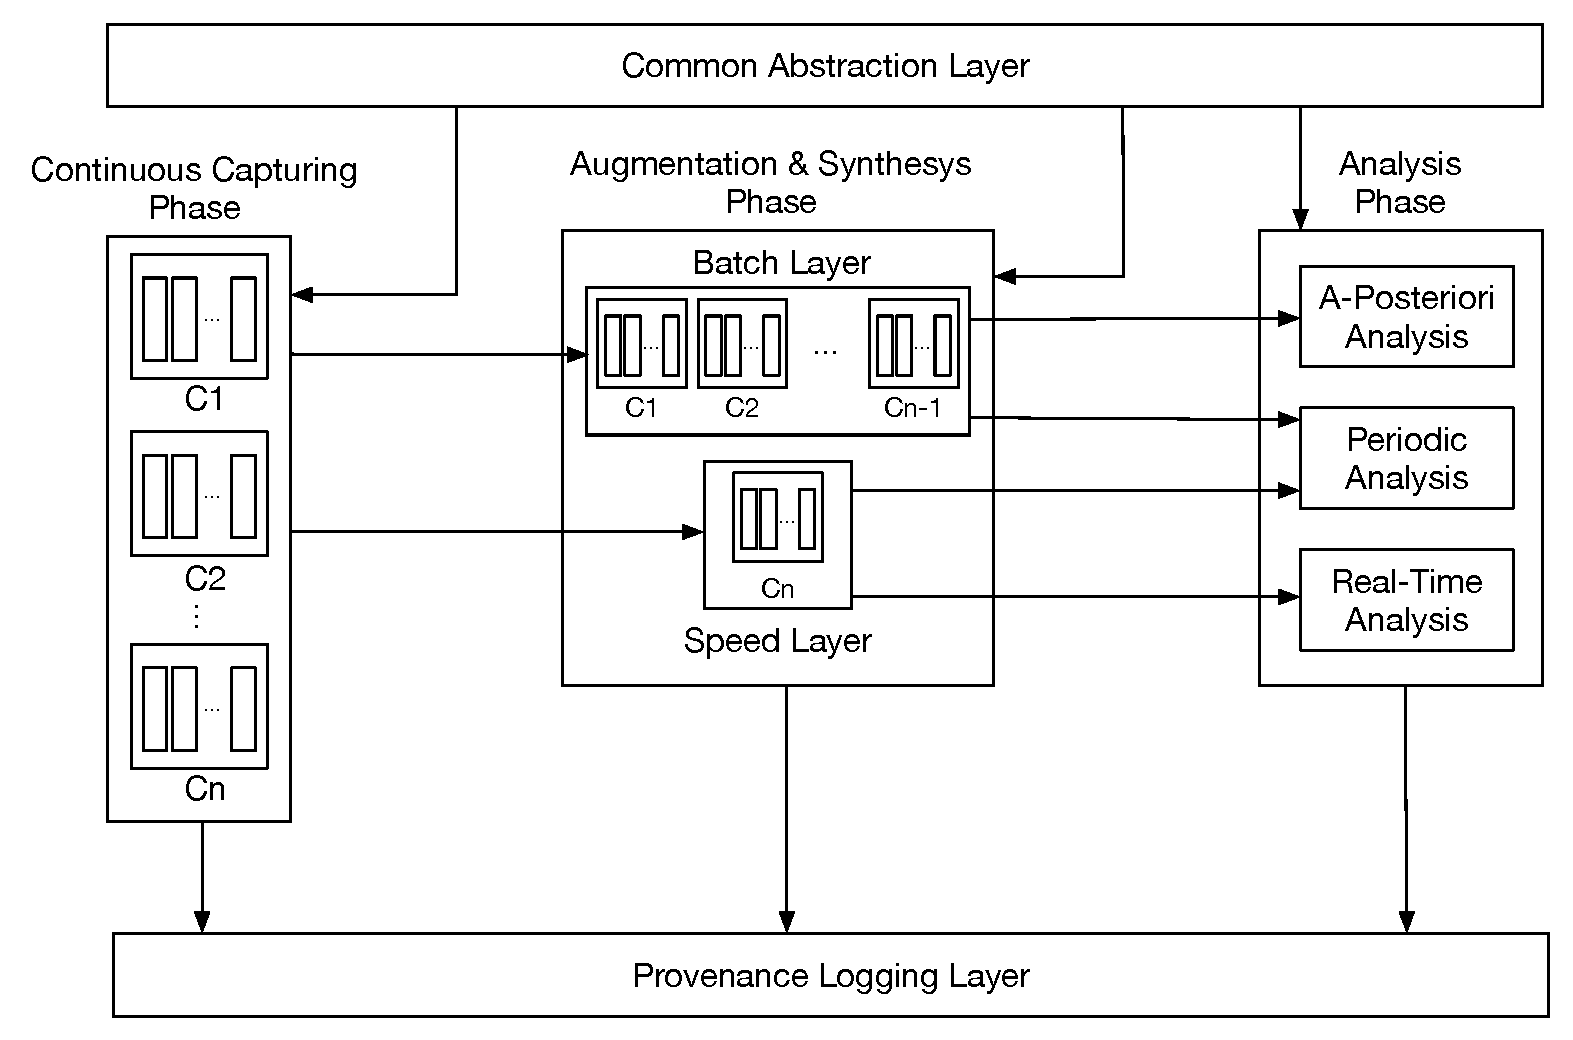
\includegraphics[width=\columnwidth]{img/computational-model-architecture}
    \caption{Example of the architecture of a system that implements \textnormal{\protect\river{}}.}
    \label{fig:arch}
\end{figure}

Figure~\ref{fig:arch} presents an reference architecture for systems that implement \river{} computational model. Information enters from the left and exits to the right going through three operational phases. 
Phase~1 (namely, Continuous Capturing Phase) continuously captures data over time. 
Phase~2 (namely, Augmentation and Synthesis Phases) enriches, manipulates and transforms captured data. 
Phase~3 (namely, Analysis Phase) analyses data to compute results.
Accordingly to the \river{}'s operators definition, Phase~1 exploits different implementations of the IN$\langle\mathrm{T}\rangle$ operator. 
Phase~2 exploits a combination of S2C$\langle\mathrm{T}\rangle$, C2C$\langle\mathrm{T},\mathrm{T^{\prime}}\rangle$ and C2S$\langle\mathrm{T}\rangle$ operators implementations. And, finally, Phase~3 exploits OUT$\langle\mathrm{T}\rangle$ operator implementations to emit the results.

During the Continuous Capturing Phase the data, which continuously flows in, is just marked with a timestamp, i.e., following the \textit{Lazy Transformation} approach, it is captured in its original form independently from its complexity.  

The proposed architecture treats \textit{Volume} as orthogonal to \textit{Variety} and \textit{Velocity}. When \textit{Volume} is present, system must implement the continuous ingestion phase in a partition tolerant way (see Section \ref{ch:computational-impl}). 

The fragment of the architecture, which has in charge the Augmentation and Synthesis Phases, is inspired by a $\lambda$ architecture (see Section~\ref{sec:vel-arch}). 
Let us denote with C$_i$ the information the Speed Layer is able to process while staying reactive, and let us denote with C$_n$ the most recently captured information, and with C$_1$, ..., C$_{n-1}$ all the data captured. While the Speed Layer processes C$_n$, the Batch Layer updates C$_1$, ..., C$_{n-2}$ with the results generated by the Speed Layer while processing C$_{n-1}$.

The Analysis Phase exploits, based on the information need of the user, indifferently various part of the upstream architecture. The Batch Layer can be used alone for periodic and post-hoc analysis, or in support of the Speed Layer for analysis that needs to compare the most recent data with the historical one. Nevertheless, the speed layer, can be independently used to perform instantaneous analysis.

For instance, a taxi company can exploit the Batch Layer, to synthesize statistics about the cost and the duration of all the rides captured so far in a city. An a-posteriori analysis of those statistics can determine a complete origin-destination matrix for the taxi rides, i.e., a distribution of the durations and the prices of all possible routes from any point to any other point in the city (see Section~\ref{sec:conc-fr-1-synth-ex}). At the same time, the taxi company can exploit the Speed Layer to determine the current most profitable routes using the latest incoming data. The comparison between the latest price of the rides (computed in the Speed Layer) with the information in the origin-destination matrix (computed in the Batch Layer) can be useful to foil a fraud.  

Two more layers compose the proposed architecture: the Common Abstraction Layer -- that contains the abstraction used to model or manipulate data (e.g., \frappe{} concepts and \river{}'s operators) and enables OBDA operations -- and the Provenance Logging Layer -- that contains all the artifact useful to document data lineage and to log the system actions (e.g., in accordance with concepts in the Provenance fragment of \frappe{}).

\section{Conclusion}
In this chapter, we investigate the problem of managing data characterized by high variety and velocity without forgetting volume.
Taking in account the conceptual model presented in Chapter~\ref{ch:conceptual}, we concentrate our efforts on the creation of a computational model to deal with data with such characteristics.

We propose \river{}, a variety-proof streaming computational model based on two main principles (see Section~\ref{sec:comp-mod-sol}): \textbf{(P1)} everything is a data stream, and \textbf{(P2)} Continuous Ingestion.
A system based on \textbf{(P1)} and \textbf{(P2)} can manage flowing data without any data loss.
During this research work, in order to answer the research question, we propose the \textit{Lazy Transformation} and formulate the hypothesis \textsf{Hp.2.1}.
A system, which implements the \textit{Lazy Transformation} approach, postpones the data transformation until it can benefit from it.

We present a formal definition of \river{}'s operators in terms of semantics and textual syntax (see Section~\ref{sec:comp-mod-sol-lang}), together with the Pipeline Definition Language (PDL) -- a graphic language that enables user to create computational plans, in the form of pipelines, to ingest, process and emit data.

\river{} represents the formal basis of the implementations proposed in the next chapter (see Chapter~\ref{ch:computational-impl}), that will be exploited to experimentally validate \textsf{Hp.2.1}.